\documentclass{zjusct-beamer/zjusctbeamer}

% Metadata
\title{A First Look at the CPU Parallel Programming Framework}
\subtitle{PM - C++ Concurrency in Action}
\author[bowling233]{Baolin Zhu (@bowling233)}
\date{\today}
\institute[ZJUSCT]{Zhejiang University Supercomputing Team}
\copyleftnotice{CC-BY 4.0}{}

\hypersetup{
    pdftitle={\title},
    pdfpagemode=FullScreen,
}

\setminted{
    fontsize=\tiny % 设置代码和行号的字体大小
}

\begin{document}

% Set Mono and Emoji font
\setmonofont{DejaVu Sans Mono}
\setemojifont{TwemojiMozilla}

\maketitle

% Outline (Table of Contents)
%\cutoc

% Slide 正文均使用英文
\section{Introduction}

% 我的简介
\begin{frame}[fragile]{\emoji{bust-in-silhouette} Biography}
	\begin{center}
		\begin{itemize}
			\item \textbf{Baolin Zhu} (\emoji{bowling} @bowling233)
			\item (with Eric) Leader of ZJUSCT
			\item \textbf{Research Interests}: Arch/OS, Three Pillars (Compute, Network and Storage)
		\end{itemize}
		\begin{tikzpicture}
			% Timeline base line
			\draw[thick, gray] (0,0) -- (10.5,0);

			% Node 0: CKC AGC
			\fill[blue] (1.5, 0) circle (0.1);
			\draw[gray] (1.5, 0) -- (1.5, 0.5);
			\node at (1.5, 1) {
\includegraphics[width=0.8cm]{day8_pm/img/bio-ckcagc}};
			\node[font=\bfseries\small] at (1.5, 2) {CKC AGC};
			\node[font=\footnotesize, gray] at (1.5, -0.5) {Freshman};

			% Node 1: ZJUSCT
			\fill[blue] (4.0, 0) circle (0.1);
			\draw[gray] (4.0, 0) -- (4, 0.5);
			\node at (4.0, 1) {
\includegraphics[width=0.8cm]{day8_pm/img/bio-zjusct}};
			\node[font=\bfseries\small] at (4.0, 2) {ZJUSCT};
			\node[font=\footnotesize, gray] at (4.0, -0.5) {Sophomore};

			% Node 2: RC4ML Lab
			\fill[blue] (6.5, 0) circle (0.1);
			\draw[gray] (6.5, 0) -- (6.5, 0.5);
			\node at (6.5, 1) {
\includegraphics[width=0.8cm]{day8_pm/img/bio-rc4ml}};
			\node[font=\bfseries\small] at (6.5, 2) {RC4ML Lab};
			\node[font=\footnotesize, gray] at (6.5, -0.5) {Junior};

			% Node 3: Tencent
			\fill[blue] (9.0, 0) circle (0.1);
			\draw[gray] (9.0, 0) -- (9.0, 0.5);
			\node at (9.0, 1) {
\includegraphics[width=0.8cm]{day8_pm/img/bio-csig}};
			\node[font=\bfseries\small] at (9.0, 2) {Tencent CSIG};
			\node[font=\footnotesize, gray] at (9.0, -0.5) {Junior};

		\end{tikzpicture}
	\end{center}
\end{frame}

% 为什么学习 C++ 并行编程:减轻心智负担
\begin{frame}[fragile]{\emoji{question} Why C++ Concurrency?}
	Reducing cognitive overhead for \textbf{application-level} (rather than systems-level) programming.
	\begin{itemize}
		\item Object-Oriented Programming (OOP) \& Encapsulation
		\item Resource Management \& RAII: Smart pointers
		\item Templates \& Generic Programming
		\item Standard Template Library (STL) \& Abstractions
		\item Safer Concurrency Models
		\item Enhanced Type Safety \& Expressiveness: References, Function Overloading, and Lambdas
	\end{itemize}
\end{frame}

% 本节课的参考教材
\begin{frame}[fragile]{\emoji{books} Textbook}

	\begin{columns}
		\begin{column}{0.4\textwidth}
			\begin{center}
				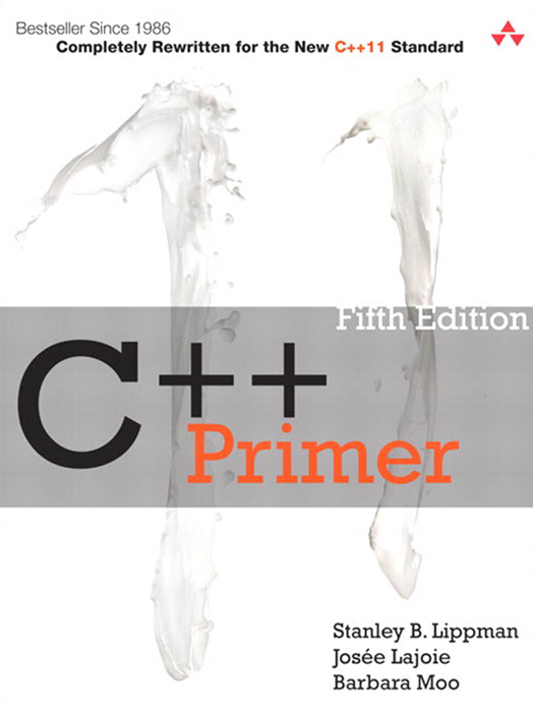
\includegraphics[width=0.8\textwidth]{day8_pm/img/1-cppprimer}
			\end{center}

		\end{column}
		\begin{column}{0.6\textwidth}
			\begin{itemize}
				\item \textbf{Title}: C++ Primer (Fifth Edition)
				\item \textbf{Authors}: Stanley B. Lippman, Josée Lajoie, and Barbara E. Moo
				\item \textbf{Publisher}: Addison-Wesley Professional
			\end{itemize}
		\end{column}
	\end{columns}
\end{frame}

\begin{frame}[fragile]{\emoji{books} Textbook}

	\begin{columns}
		\begin{column}{0.4\textwidth}
			\begin{center}
				
\includegraphics[width=0.8\textwidth]{day8_pm/img/1-ccia}
			\end{center}

		\end{column}
		\begin{column}{0.6\textwidth}
			\begin{itemize}
				\item \textbf{Title}: C++ Concurrency in Action (Second Edition)
				\item \textbf{Authors}: Anthony Williams
				\item \textbf{Publisher}: Manning Publications
			\end{itemize}
		\end{column}
	\end{columns}
\end{frame}

% Tips:遇到 C/C++ 语法问题,去 CPPREFERENCE 查找
\begin{frame}[fragile]{\emoji{light-bulb} Tips}
	\begin{itemize}
		\item \textbf{C/C++ Reference}: Use \textcolor{blue}{\href{https://en.cppreference.com/}{cppreference}} for syntax and library functions
		\item \textbf{Compiler Documentation}: Check your compiler's documentation for specific features and extensions (Example: \textcolor{blue}{\href{https://gcc.gnu.org/onlinedocs/gcc/Attributes.html}{GCC Attributes}})
		\item \textbf{Online Communities}: Engage with communities like Stack Overflow for troubleshooting and best practices
	\end{itemize}
\end{frame}

% 本节课的内容大纲
\begin{frame}[fragile]{\emoji{book} Outline}
	\begin{enumerate}
		\item \textbf{C++ Quick Start}
		      \begin{itemize}
			      \item Key differences between C++ and C
				  \item Object-oriented programming
				  \item Containers and Algorithms
		      \end{itemize}
		\item \textbf{C++ Concurrency Overview}
		      \begin{itemize}
			      \item Comparison: OpenMP, MPI, C++ threads
			      \item Thread lifecycle management
		      \end{itemize}
		\item \textbf{Shared Data Synchronization}
		      \begin{itemize}
			      \item From C mutexes to C++ RAII locks
			      \item Deadlock prevention strategies
		      \end{itemize}
		\item \textbf{Producer-Consumer Model}
		      \begin{itemize}
			      \item Condition variables and thread-safe queues
			      \item Practical implementation
		      \end{itemize}
		\item \textbf{Summary and Framework Selection}
		      \begin{itemize}
			      \item Comprehensive comparison and use cases
			      \item Monte Carlo π calculation example
		      \end{itemize}
	\end{enumerate}
\end{frame}

% 预修要求:C 语言,否则请先跳过本节课,补习 C 语言基础
\begin{frame}[fragile]{\emoji{warning} Prerequisites}
	\begin{itemize}
		\item \textbf{C Language Proficiency}: Basic understanding of C syntax and concepts
		\item \textbf{Familiarity with Pointers}: Understanding of pointers, memory management, and basic data structures
		\item \textbf{Basic Programming Constructs}: Loops, conditionals, functions, and arrays
	\end{itemize}
\end{frame}

\section{C++ Quick Start}

\subsection{Object-Oriented Programming}

% 简单对比过程式编程和面向对象编程
\begin{frame}[fragile]{Procedural vs Object-Oriented Programming}
    \begin{columns}
        \begin{column}{0.5\textwidth}
            \textbf{C: Procedural Programming}
            \begin{itemize}
                \item Focus on functions and data
                \item Functions operate on data structures
                \item No built-in support for encapsulation or inheritance
            \end{itemize}
        \end{column}
        \begin{column}{0.5\textwidth}
            \textbf{C++: Object-Oriented Programming}
            \begin{itemize}
                \item Combines data and functions into classes
                \item Supports encapsulation, inheritance, and polymorphism
                \item Provides a more modular and reusable code structure
            \end{itemize}
        \end{column}
    \end{columns}

    A class defines a type \textbf{along with a collection of operations that are related to that type}.
\end{frame}

\begin{frame}[fragile]{Procedural vs Object-Oriented Programming}
	\begin{columns}
		\begin{column}{0.5\textwidth}
			\textbf{C Struct (Data \textcolor{orange}{and} Functions)}
			\begin{minted}{c}
struct Student {
    char name[50];
    int age;
    float gpa;
};
void print_student(struct Student s) {
    printf("Name: %s\n", s.name);
    printf("Age: %d\n", s.age);
    printf("GPA: %.2f\n", s.gpa);
}
int main() {
    struct Student alice = {"Alice", 20, 3.8};
    print_student(alice);
    return 0;
}
			\end{minted}
		\end{column}
		\begin{column}{0.5\textwidth}
			\textbf{C++ Class (Data \textcolor{orange}{with} Functions)}
			\begin{minted}{cpp}
class Student {
private:
    string name;
    int age;
    float gpa;
public:
    Student(string n, int a, float g)
        : name(n), age(a), gpa(g) {}
    void print() {
        cout << "Name: " << name << endl;
        cout << "Age: " << age << endl;
        cout << "GPA: " << gpa << endl;
    }
};
int main() {
    Student alice("Alice", 20, 3.8);
    alice.print();  // Object calls its own method
    return 0;
}
			\end{minted}
		\end{column}
	\end{columns}
\end{frame}

\begin{frame}[fragile]{Abstract Data Types}
    The fundamental ideas behind classes are \textbf{data abstraction} and \textbf{encapsulation}.

    \begin{itemize}
        \item \textbf{Data Abstraction}: Separation of \textcolor{blue}{interface} and \textcolor{orange}{implementation}
        \item \textbf{Encapsulation}: Enforces this separation by hiding implementation details
        \item Together, they define an \textbf{Abstract Data Type (ADT)}
    \end{itemize}

    \vspace{0.3em}
    \begin{columns}
        \begin{column}{0.5\textwidth}
            \textbf{Interface (What users see)}
            \begin{itemize}
                \item Public operations users can execute
                \item Contract of what the class does
                \item Think abstractly about behavior
            \end{itemize}
        \end{column}
        \begin{column}{0.5\textwidth}
            \textbf{Implementation (Hidden details)}
            \begin{itemize}
                \item Data members
                \item Function bodies
                \item Internal helper functions
            \end{itemize}
        \end{column}
    \end{columns}
\end{frame}

\begin{frame}[fragile]{Abstract Data Type: An Example}
    \begin{columns}
        \begin{column}{0.5\textwidth}
        \textbf{Interface (Public)}
            \begin{itemize}
                \item \texttt{Book(title, author, pages, count)} - Constructor
                \item \texttt{isAvailable()} - Check availability
                \item \texttt{addCopies(num)} - Add copies
            \end{itemize}
            \vspace{0.3em}
            \textbf{Users care about:} \\
            \textit{What} operations are available, not \textit{how} they work
        \end{column}
        \begin{column}{0.5\textwidth}
            \begin{minted}{cpp}
class Book {
private:  // Implementation (Hidden)
    string title;
    string author;
    int pages;
    int count;
public:   // Interface (Visible)
    Book(string t, string a, int p, int c);
    bool isAvailable() const;
    void addCopies(int num);
};
            \end{minted}
        \end{column}
    \end{columns}
\end{frame}

\begin{frame}[fragile]{Abstract Data Types: Key Benefits}

    \begin{columns}
        \begin{column}{0.5\textwidth}
            \textbf{For Class Designers:}
            \begin{itemize}
                \item Focus on \textbf{how} the class is implemented
                \item Can change implementation without breaking user code
                \item Control access to internal data
            \end{itemize}
        \end{column}
        \begin{column}{0.5\textwidth}
            \textbf{For Class Users:}
            \begin{itemize}
                \item Don't need to know \textbf{how} the type works
                \item Think abstractly about \textbf{what} the type does
                \item Use the interface without worrying about details
            \end{itemize}
        \end{column}
    \end{columns}
\end{frame}

\begin{frame}[fragile]{Class: Definition}
    \begin{minted}[fontsize=\scriptsize]{cpp}
class ClassName {
public:  // Public interface
    ClassName();  // Constructor
    ~ClassName(); // Destructor
    void publicMethod();  // Public method
private: // Private implementation details
    int privateData;  // Private data member
    void privateMethod();  // Private method
protected: // Protected members (accessible by derived classes)
    int protectedData;  // Protected data member
};
    \end{minted}
\end{frame}


\begin{frame}[fragile]{Class: \texttt{this} pointer}
    \textbf{The \texttt{this} pointer:} A special pointer that refers to the current object

    \begin{itemize}
        \item Used inside class methods to access members of the current object
        \item Helps distinguish between member variables and parameters with the same name
    \end{itemize}

    \textbf{Example:}
    \begin{minted}{cpp}
class Point {
private:
    int x, y;
public:
    Point(int x, int y) {
        this->x = x;  // Use this to refer to member variable
        this->y = y;  // Use this to refer to member variable
    }
};
    \end{minted}
\end{frame}


\begin{frame}[fragile]{Encapsulation}
	\textbf{Encapsulation enforces the separation of interface and implementation}
	\begin{itemize}
		\item \textbf{Hide Implementation}: Users cannot access internal details
		\item \textbf{Control Access}: Define exactly how others can use your class
		\item \textbf{Maintainability}: Change implementation without breaking user code
		\item \textbf{Data Protection}: Prevent accidental or malicious modification
	\end{itemize}

\end{frame}

\begin{frame}[fragile]{Encapsulation: Access specifiers}
	\begin{minted}[fontsize=\scriptsize]{cpp}
class BankAccount {
private:    // Only this class can access
    double balance;
public:     // Anyone can access
    void deposit(double amount) {
        if (amount > 0) balance += amount;  // Safe deposit
    }
    double getBalance() const { return balance; }  // Read-only access
protected:  // This class and its children can access
    void setBalance(double newBalance) { balance = newBalance; }
};
    \end{minted}
    \begin{itemize}
        \item \texttt{struct}: Members are \textbf{public} by default - less encapsulation
        \item \texttt{class}: Members are \textbf{private} by default - enforces encapsulation
    \end{itemize}
\end{frame}

\begin{frame}[fragile]{Inheritance: Building on Existing Code}
	\textbf{Like a Family Tree:} Children inherit traits from parents

	\begin{columns}
		\begin{column}{0.3\textwidth}
			\textbf{Base Class (Parent)}
			\begin{minted}{cpp}
class Animal {
protected:
    string name;
public:
    Animal(string n) : name(n) {}
    void eat() { cout << name << " is eating\n"; }
    virtual void makeSound() { cout << name << " makes a sound\n"; }
};
    \end{minted}
		\end{column}
		\begin{column}{0.7\textwidth}
			\textbf{Derived Class (Child)}
			\begin{minted}{cpp}
class Dog : public Animal {
public:
    Dog(string n) : Animal(n) {}  // Call parent constructor
    void makeSound() override {        // Override parent method
        cout << name << " barks: Woof!\n";
    }
    void wagTail() { cout << name << " wags tail\n"; }  // New method
};

int main() {
    Dog buddy("Buddy");
    buddy.eat();        // Inherited from Animal
    buddy.makeSound();  // Dog's own version
    buddy.wagTail();    // Dog-specific behavior
    return 0;
}
    \end{minted}
		\end{column}
	\end{columns}
\end{frame}

\begin{frame}[fragile]{Polymorphism: One Interface, Many Forms}
	\textbf{Like a Universal Remote:} Same buttons, different devices

	\begin{columns}
		\begin{column}{0.6\textwidth}
			\begin{minted}{cpp}
class Shape {
public:
    virtual double area() = 0;  // Pure virtual function
    virtual ~Shape() = default;
};
class Circle : public Shape {
    double radius;
public:
    Circle(double r) : radius(r) {}
    double area() override { return 3.14159 * radius * radius; }
};
class Rectangle : public Shape {
    double width, height;
public:
    Rectangle(double w, double h) : width(w), height(h) {}
    double area() override { return width * height; }
};
    \end{minted}
		\end{column}
		\begin{column}{0.4\textwidth}

			\begin{minted}{cpp}
vector<unique_ptr<Shape>> shapes;
shapes.push_back(make_unique<Circle>(5.0));
shapes.push_back(
    make_unique<Rectangle>(4.0, 6.0));
for (auto& shape : shapes) {
    cout << "Area: " << shape->area()
         << endl;
    // Calls correct method
}
    \end{minted}
		\end{column}
	\end{columns}
\end{frame}

\subsection{The Basics}

\begin{frame}[fragile]{I/O Streams: Compared to C Standard I/O}
	\begin{columns}
		\begin{column}{0.5\textwidth}
			\textbf{C Style}
			\begin{minted}{c}
#include <stdio.h>
#include <stdlib.h>

void print_msg(void) {
    printf("Hello from C!\n");
}

int main() {
    FILE* fp = fopen("test.txt", "r");
    if (fp) {
        // Manual resource management
        char line[100];
        while (fgets(line, 100, fp) != NULL) {
            printf("%s", line);
        }
        fclose(fp);
    }
    return 0;
}
			\end{minted}
		\end{column}
		\begin{column}{0.5\textwidth}
			\textbf{C++ Style}
			\begin{minted}{cpp}
#include <iostream>
#include <fstream>

void print_msg() {
    std::cout << "Hello from C++!" << std::endl;
}

int main() {
    std::ifstream file("test.txt");
    if (file.is_open()) {
        // Automatic resource management
        std::string line;
        while (std::getline(file, line)) {
            std::cout << line << std::endl;
        }
    }
    return 0;
}
			\end{minted}
		\end{column}
	\end{columns}
\end{frame}

% 介绍 C++ 的引用和指针
\begin{frame}[fragile]{References}
	\begin{columns}
		\begin{column}{0.5\textwidth}
			\textbf{C Pointers}
			\begin{minted}{c}
void swap_c(int* a, int* b) {
    int temp = *a;
    *a = *b;
    *b = temp;
}
int main() {
    int x = 5, y = 10;
    swap_c(&x, &y);  // Pass addresses
    printf("x=%d, y=%d\n", x, y);
    return 0;
}
			\end{minted}
		\end{column}
		\begin{column}{0.5\textwidth}
			\textbf{C++ References}
			\begin{minted}{cpp}
void swap_cpp(int& a, int& b) {
    int temp = a;
    a = b;
    b = temp;
}
int main() {
    int x = 5, y = 10;
    swap_cpp(x, y);  // Direct pass
    cout << "x=" << x << ", y=" << y << endl;
    return 0;
}
			\end{minted}
		\end{column}
	\end{columns}

	\vspace{0.5em}
	\begin{itemize}
		\item References are \textbf{aliases} for existing objects: \texttt{int a; int\& b = a;}
		\item References must be initialized and cannot be reassigned
	\end{itemize}
\end{frame}

% 本页展示 C++ 的所有运算符
\begin{frame}[fragile]{C++ Operators and Keywords (From \textcolor{blue}{\href{https://en.cppreference.com/w/cpp/language/}{cppreference.com}})}
	\begin{columns}
		\begin{column}{0.6\textwidth}
			\begin{figure}
				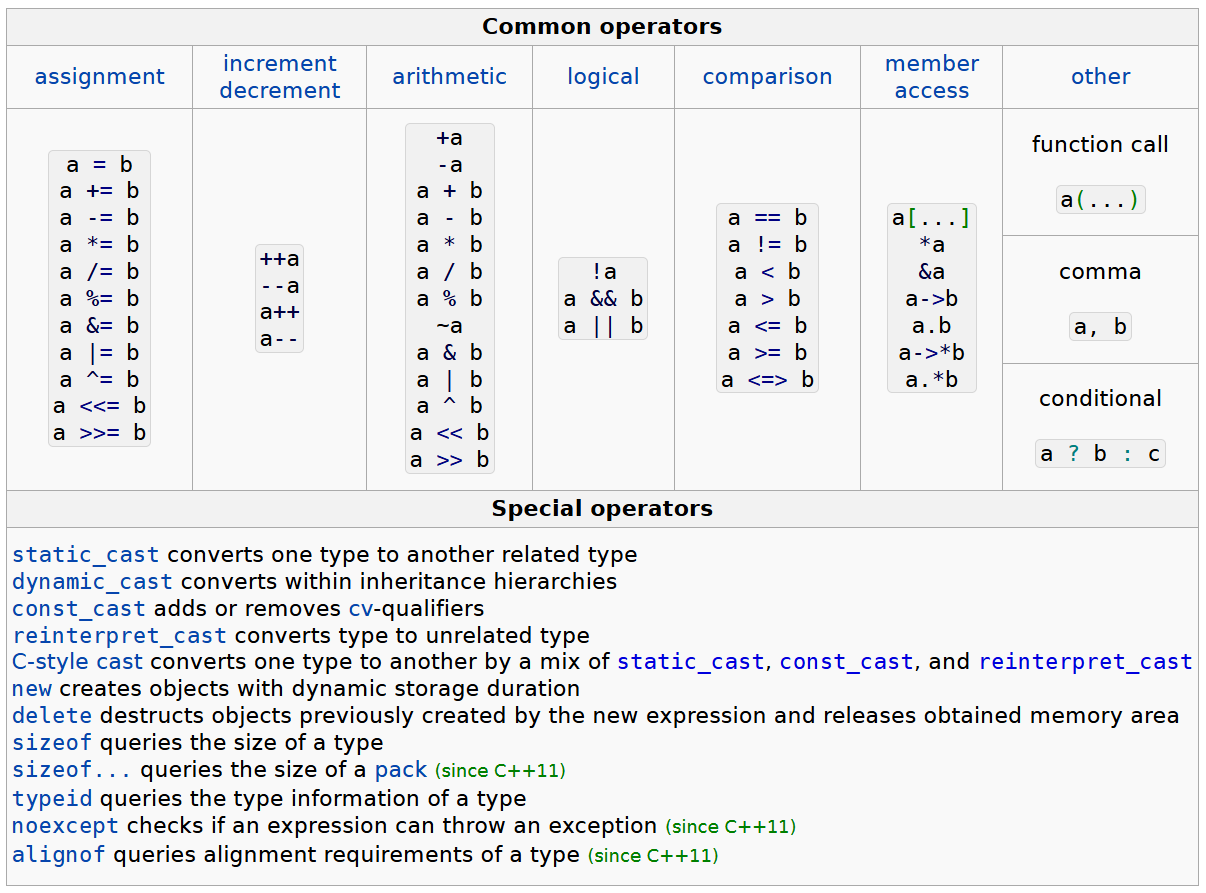
\includegraphics[width=\textwidth]{day8_pm/img/1-operators}
			\end{figure}
		\end{column}
		\begin{column}{0.4\textwidth}
			\begin{figure}
				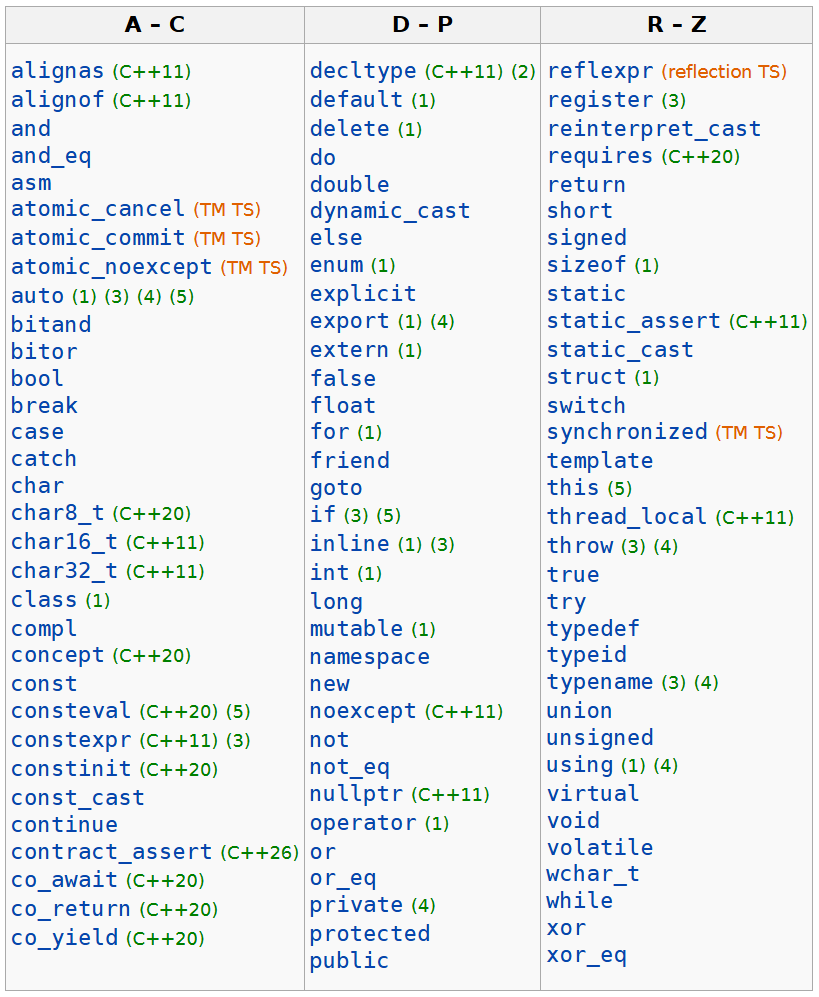
\includegraphics[width=0.9\textwidth]{day8_pm/img/1-keywords}
			\end{figure}
		\end{column}
	\end{columns}
\end{frame}

\begin{frame}[fragile]{C++ Operators and Keywords}
	We'll meet some new friends in this class:
	\begin{itemize}
		\item \textbf{I/O}:  \texttt{>>}, \texttt{<<}
		\item \textbf{Memory}: \texttt{new}, \texttt{delete}, \texttt{new[]}, \texttt{delete[]}
		\item \textbf{Type System}: \texttt{auto}, \texttt{decltype}, \texttt{using}, \texttt{operator}
		\item \textbf{Class}: \texttt{::}, \texttt{public}, \texttt{private}, \texttt{protected}, \texttt{friend}, \texttt{virtual}, \texttt{override}, \texttt{final}
	\end{itemize}
\end{frame}

% 上页给出代码对比,本页给出讲解
\begin{frame}[fragile]{I/O Streams}
    \begin{table}[]
        % table of streams: i, o, io; file, string, c
        \begin{tabular}{cccc}
            \hline
            \textbf{Type} & \textbf{Input} & \textbf{Output} & \textbf{Both} \\ \hline
            standard & \texttt{cin} & \texttt{cout}, \texttt{cerr}, \texttt{clog} &  \\ \hline
            File         & \texttt{ifstream} & \texttt{ofstream} & \texttt{fstream} \\ \hline
            String       & \texttt{istringstream} & \texttt{ostringstream} & \texttt{stringstream} \\ \hline
        \end{tabular}
    \end{table}

	\textbf{Benefits of C++ Streams:}
	\begin{itemize}
		\item Type safety and flexibility
		\item Easier to read and maintain code
		\item Automatic resource cleanup when objects go out of scope
	\end{itemize}
\end{frame}

% 给出一个 sstream 的例子,以展示相比 C 的优势
\begin{frame}[fragile]{I/O Streams: Example}
    \textbf{String Streams:} Like a string that can be read/written like a file
    \begin{minted}{cpp}
#include <sstream>
#include <iostream>

void example_string_stream() {
    std::stringstream ss;
    ss << "The answer is " << 42;
    std::string result = ss.str();
    std::cout << result << std::endl;
}
    \end{minted}

    \textbf{Benefits:}
    \begin{itemize}
        \item Concise syntax for formatting strings
        \item No need for manual memory management
        \item Can be used with any type that supports stream operators
    \end{itemize}
\end{frame}

% 介绍命名空间,标准库的所有名字都在命名空间 std 中
\begin{frame}[fragile]{Namespaces}
	\begin{itemize}
		\item C++ uses namespaces to avoid \textbf{name collisions}
		\item \textbf{Standard library} functions and classes are in the \texttt{std} namespace
		\item Use \texttt{using namespace std;} to avoid prefixing with \texttt{std::} (should be avoided in header files and large projects)
	\end{itemize}
	\textbf{Example:}
	\begin{minted}[fontsize=\scriptsize]{cpp}
#include <iostream>
using namespace std;
cout << "Hello, World!" << endl;
        \end{minted}
\end{frame}

% 介绍运算符语法
\begin{frame}[fragile]{Class: Operator overloading}
	\begin{itemize}
        \item C++ lets us define what the operators mean \textbf{when applied to objects of class type}.
		\item They are \textbf{special functions} with concise syntax
		\item Can be \textbf{overloaded} to provide custom behavior for user-defined types
        \item In a user-defined operator overload, \textbf{any type} can be used as return type (including \texttt{void})
		\item Operators for \textbf{primitive types} like \texttt{int}, \texttt{float}, etc. cannot be overloaded
	\end{itemize}

	\textbf{Syntax:}
	\begin{minted}[fontsize=\scriptsize]{cpp}
<return_type> operator<operator_symbol>(<parameters>) { /* Implementation */ }
// An illustration of overloading the + operator
int operator+(int a, int b) { return a + b; }
    \end{minted}
\end{frame}

% 以 I/O 操作符为例,介绍运算符重载:巧妙地通过重载,利用了移位运算符的语法
\begin{frame}[fragile]{Class: Operator overloading}
    \textbf{Why Overload I/O Operators?}
    \begin{itemize}
        \item Makes it easy to print custom objects
        \item Uses existing syntax (\texttt{<<} and \texttt{>>}) for a natural feel
    \end{itemize}

    \textbf{Prototype}
    % A prototype demonstrating how stream class overloads the I/O operators
    \begin{minted}{cpp}
template< class Traits >
basic_ostream<char, Traits>&
    operator<<( basic_ostream<char, Traits>& os, const char* s );
basic_istream& operator>>( int& value );
    \end{minted}
    \textbf{Example Usage}:
	\begin{minted}{cpp}
cout << "Hello, World!" << endl;
cin >> user_input;
    \end{minted}
\end{frame}

\begin{frame}[fragile]{Function Overloading: Same Name, Different Parameters}
    \textbf{Function Overloading:} Multiple functions with the same name but different parameters

    \begin{itemize}
        \item C++ allows multiple functions with the same name
        \item Functions must differ in number or type of parameters
        \item Compiler chooses the best match based on arguments
        \item Return type alone is \textbf{not} enough to distinguish functions
    \end{itemize}

    \textbf{Example:}
    \begin{minted}[fontsize=\scriptsize]{cpp}
void print(int value) {
    cout << "Integer: " << value << endl;
}
void print(double value) {
    cout << "Double: " << value << endl;
}
void print(const string& value) {
    cout << "String: " << value << endl;
}
int main() {
    print(42);        // Calls print(int)
    print(3.14);      // Calls print(double)
    print("Hello");   // Calls print(const string&)
    return 0;
}
    \end{minted}
\end{frame}

\begin{frame}[fragile]{Function Overloading vs C Naming Conventions}
    \begin{columns}
        \begin{column}{0.5\textwidth}
            \textbf{C Style: Different Names}
            \begin{minted}[fontsize=\tiny]{c}
#include <stdio.h>
#include <math.h>

// Need different names for each type
int abs_int(int x) {
    return x < 0 ? -x : x;
}
double abs_double(double x) {
    return x < 0.0 ? -x : x;
}
float abs_float(float x) {
    return x < 0.0f ? -x : x;
}

int main() {
    printf("%d\n", abs_int(-5));
    printf("%.2f\n", abs_double(-3.14));
    printf("%.2f\n", abs_float(-2.5f));
    return 0;
}
            \end{minted}
        \end{column}
        \begin{column}{0.5\textwidth}
            \textbf{C++ Style: Overloaded Functions}
            \begin{minted}[fontsize=\tiny]{cpp}
#include <iostream>
#include <cmath>
using namespace std;

// Same name, different parameters
int abs(int x) {
    return x < 0 ? -x : x;
}
double abs(double x) {
    return x < 0.0 ? -x : x;
}
float abs(float x) {
    return x < 0.0f ? -x : x;
}

int main() {
    cout << abs(-5) << endl;      // Calls abs(int)
    cout << abs(-3.14) << endl;   // Calls abs(double)
    cout << abs(-2.5f) << endl;   // Calls abs(float)
    return 0;
}
            \end{minted}
        \end{column}
    \end{columns}
\end{frame}

\begin{frame}[fragile]{Function Overloading: Rules and Best Practices}
    \textbf{Overloading Rules:}
    \begin{itemize}
        \item Functions must differ in \textbf{number} or \textbf{type} of parameters
        \item \textbf{const} and non-const parameters are considered different
        \item Reference and non-reference parameters are different
        \item Return type alone cannot distinguish overloaded functions
    \end{itemize}

    \textbf{Example of Valid Overloads:}
    \begin{minted}[fontsize=\scriptsize]{cpp}
void func(int x);                    // Version 1
void func(double x);                 // Version 2: different type
void func(int x, int y);             // Version 3: different number of parameters
void func(const int& x);             // Version 4: different parameter form
// void func(int x) { return 5; }    // ERROR: Only return type differs
    \end{minted}

    \textbf{Best Practice:} Use overloading for functions that perform \textbf{similar operations} on different types
\end{frame}

\subsection{Containers and Algorithms}
\begin{frame}[fragile]{STL: Your Programming Toolbox}
	\textbf{Standard Template Library (STL):}
	\begin{itemize}
		\item \textbf{Containers}: Ready-made data structures (like toolboxes)
		\item \textbf{Algorithms}: Common operations (like tools)
		\item \textbf{Iterators}: Ways to access container elements (like handles)
	\end{itemize}

	\vspace{0.5em}
	\textbf{Why use STL instead of arrays?}
	\begin{itemize}
		\item \textbf{Safety}: Automatic bounds checking and memory management
		\item \textbf{Convenience}: Built-in functions for common operations
		\item \textbf{Performance}: Optimized implementations
		\item \textbf{Compatibility}: Works seamlessly with C++ features
	\end{itemize}
\end{frame}

\begin{frame}[fragile]{Common Containers: Your Data Storage Options}
	\begin{columns}
		\begin{column}{0.5\textwidth}
			\textbf{Vector: Dynamic Array}
			\begin{minted}{cpp}
vector<int> numbers;
// Add elements
numbers.push_back(10);
numbers.push_back(20);
numbers.push_back(30);
// Access elements
cout << "First: " << numbers[0] << endl;
cout << "Size: " << numbers.size() << endl;
// Iterate through all
for (int num : numbers) { cout << num << " "; }
			\end{minted}
		\end{column}
		\begin{column}{0.5\textwidth}
			\textbf{Map: Key-Value Storage}
			\begin{minted}{cpp}
map<string, int> scores;
// Add key-value pairs
scores["Alice"] = 95;
scores["Bob"] = 87;
scores["Charlie"] = 92;
// Look up values
cout << "Alice's score: "
            << scores["Alice"] << endl;
// Check if key exists
if (scores.find("David") != scores.end()) {
    cout << "David found\n";
} else {
    cout << "David not found\n";
}
			\end{minted}
		\end{column}
	\end{columns}
\end{frame}

\begin{frame}[fragile]{Algorithms: Ready-Made Solutions}
	\textbf{Common algorithms you'll use:}
	\begin{table}[]
		\begin{tabular}{|l|l|}
			\hline
			\textbf{Category}       & \textbf{Algorithms}                                                                  \\ \hline
			\textbf{Sorting}        & \texttt{sort}, \texttt{stable\_sort}, \texttt{partial\_sort}, \texttt{nth\_element}  \\ \hline
			\textbf{Searching}      & \texttt{find}, \texttt{binary\_search}, \texttt{lower\_bound}, \texttt{upper\_bound} \\ \hline
			\textbf{Modifying}      & \texttt{copy}, \texttt{swap}, \texttt{replace}, \texttt{fill}, \texttt{transform}    \\ \hline
			\textbf{Set Operations} & \texttt{set\_union}, \texttt{set\_intersection}, \texttt{set\_difference}            \\ \hline
			\textbf{Numeric}        & \texttt{accumulate}, \texttt{inner\_product}, \texttt{adjacent\_difference}          \\ \hline
		\end{tabular}
	\end{table}
\end{frame}

\begin{frame}[fragile]{Algorithms: Ready-Made Solutions}
	\begin{minted}[fontsize=\scriptsize]{cpp}
vector<int> numbers = {64, 34, 25, 12, 22, 11, 90};
// Sort the vector
sort(numbers.begin(), numbers.end());
cout << "Sorted: ";
for (int n : numbers) cout << n << " ";
cout << endl;
// Find an element
auto it = find(numbers.begin(), numbers.end(), 25);
if (it != numbers.end()) {
    cout << "Found 25 at position: "
                << (it - numbers.begin()) << endl;
}
// Count elements greater than 30
int count = count_if(numbers.begin(), numbers.end(),
    [](int n) { return n > 30; });
cout << "Numbers > 30: " << count << endl;
    \end{minted}
\end{frame}

\begin{frame}[fragile]{More on STL Algorithms}
	\begin{figure}
		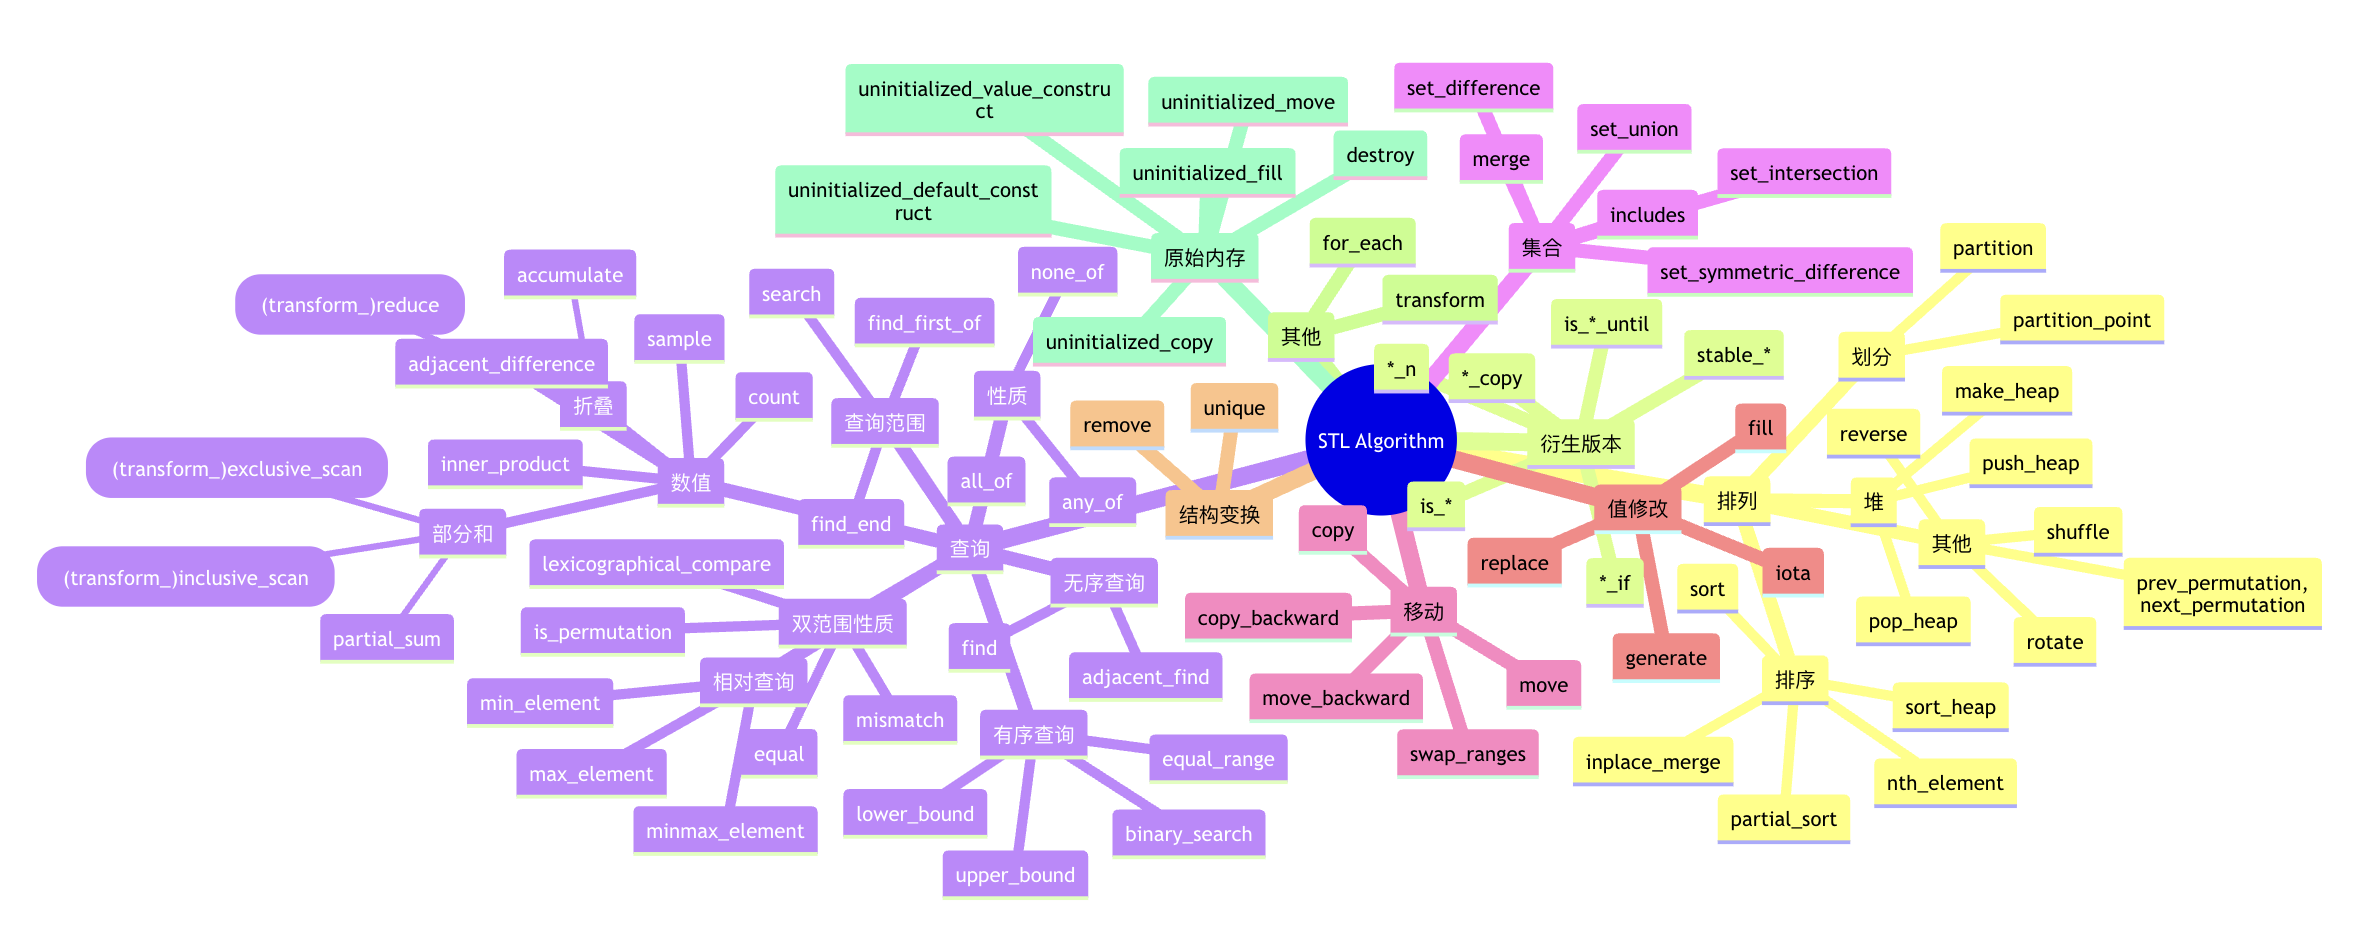
\includegraphics[width=\textwidth]{day8_pm/img/2-algorithms}
	\end{figure}
\end{frame}

\begin{frame}[fragile]{More on STL Algorithms}
	\textcolor{blue}{\href{https://www.youtube.com/watch?v=2olsGf6JIkU&ab_channel=CppCon}{CppCon 2018: 105 STL Algorithms in Less Than an Hour}}
	\begin{figure}
		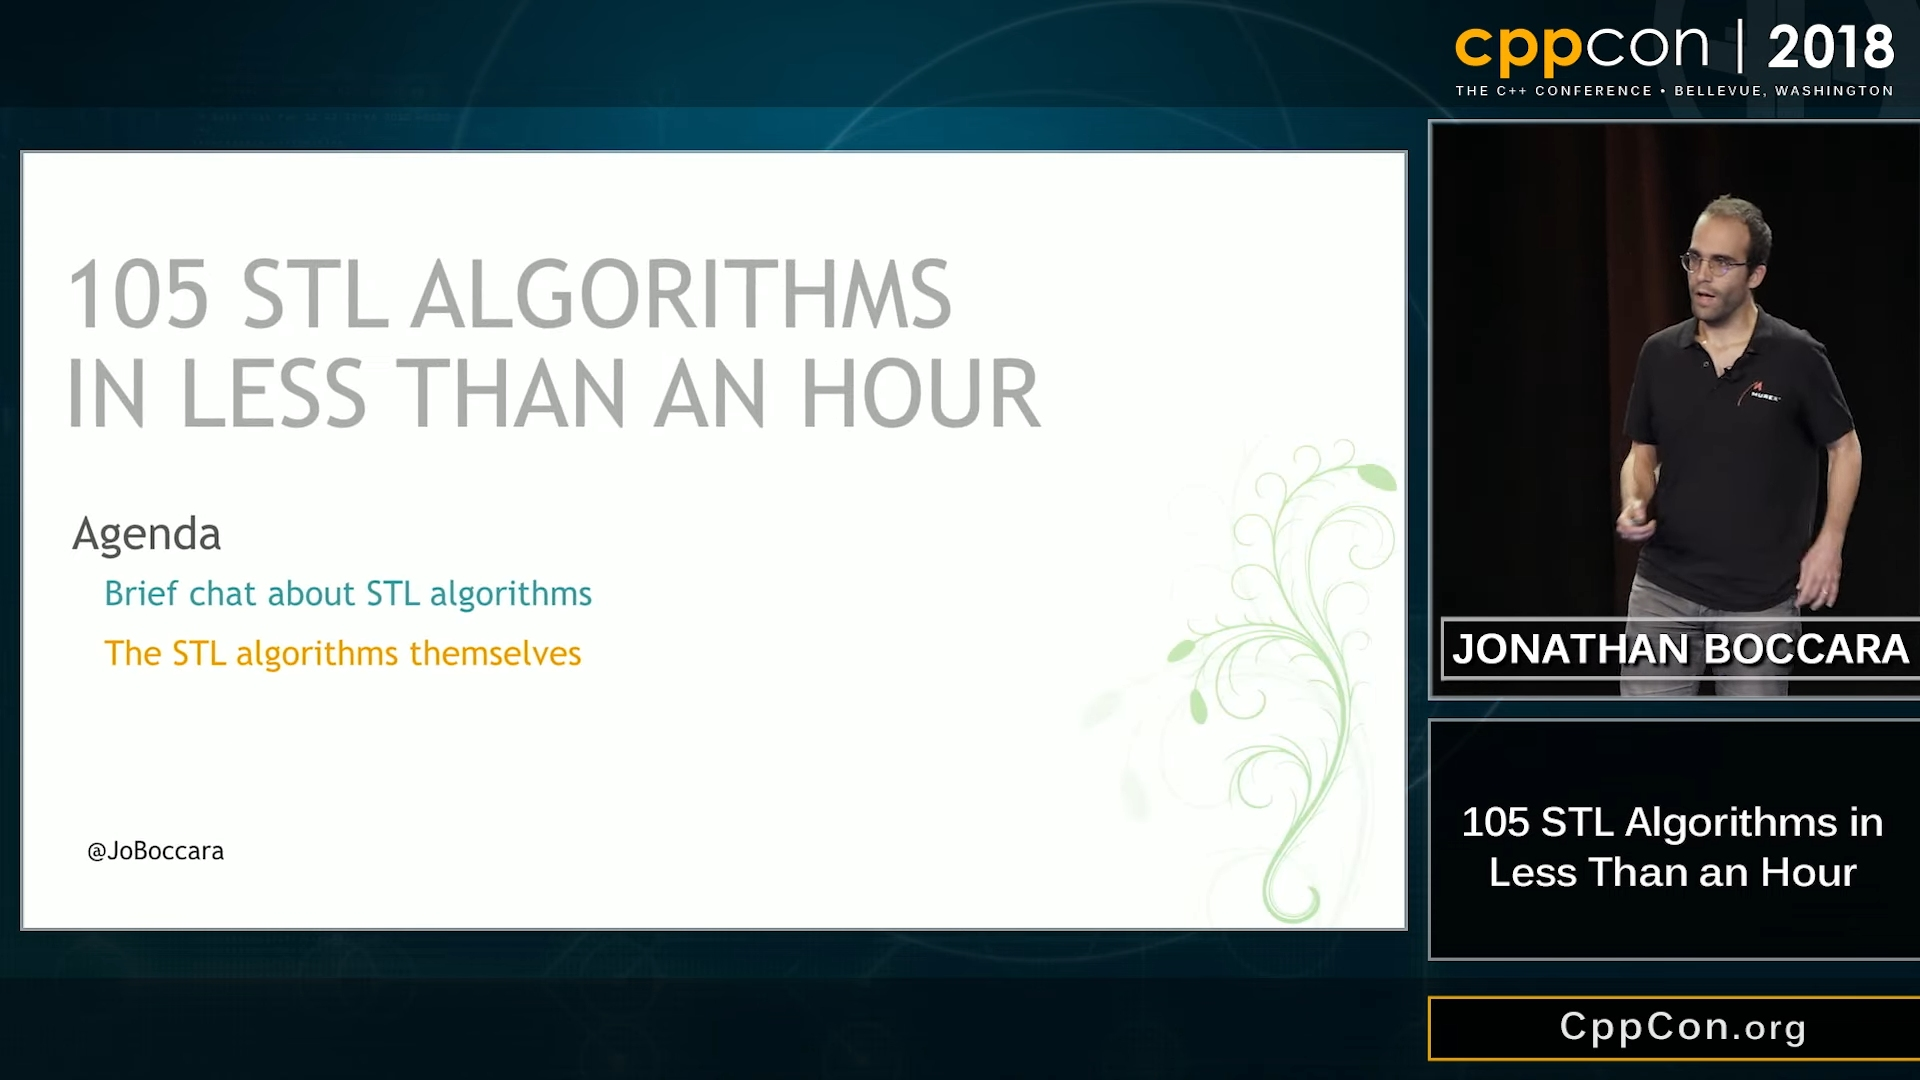
\includegraphics[width=0.7\textwidth]{day8_pm/img/2-cppcon2018}
	\end{figure}
\end{frame}

\begin{frame}[fragile]{Containers vs C Arrays: The Upgrade}
	\begin{columns}
		\begin{column}{0.5\textwidth}
			\textbf{C Arrays (Manual Everything)}
			\begin{minted}{c}
int arr[] = {1, 3, 2};
int size = 0;
// must write your compare function
qsort(ints, size, sizeof(int), compare_ints);
for (int i = 0; i < size; i++) {
    printf("%d ", arr[i]);
}
			\end{minted}
		\end{column}
		\begin{column}{0.5\textwidth}
			\textbf{C++ Containers (Automatic)}
			\begin{minted}{cpp}
// Dynamic size, automatic memory
vector<int> arr = {1, 3, 2};
sort(arr.begin(), arr.end());
for (int num : arr) {
    cout << num << " ";
}
			\end{minted}
		\end{column}
	\end{columns}

	\vspace{0.5em}
	\textbf{Benefits:} Safer, shorter, and often faster code!
\end{frame}

\subsection{Essential Features for Concurrency}
\begin{frame}[fragile]{Callable Objects}
    \textbf{Function Call Operator}
    \begin{minted}{cpp}
function (arg1, arg2, arg3,...)
    \end{minted}

    \textbf{Callable Object}
    \begin{itemize}
        \item An object that can be called like a function
        \item Functions and pointers to functions, \textbf{lambdas}, objects created by bind, and \textbf{classes that overload the function-call operator}.
    \end{itemize}
\end{frame}

\begin{frame}[fragile]{Lambda Expressions: The Core of Thread Functions}
	\begin{columns}
		\begin{column}{0.5\textwidth}
			\textbf{C Function Pointers}
			\begin{minted}{c}
#include <pthread.h>

void* thread_func(void* arg) {
    int id = *(int*)arg;
    printf("Thread %d running\n", id);
    return NULL;
}

int main() {
    pthread_t thread;
    int id = 1;
    pthread_create(&thread, NULL,
                   thread_func, &id);
    pthread_join(thread, NULL);
    return 0;
}
			\end{minted}
		\end{column}
		\begin{column}{0.5\textwidth}
			\textbf{C++ Lambda}
			\begin{minted}{cpp}
#include <thread>
#include <iostream>

int main() {
    int id = 1;

    // Lambda expression
    auto thread_func = [id]() {
        cout << "Thread " << id
                  << " running" << endl;
    };

    thread t(thread_func);
    t.join();

    return 0;
}
			\end{minted}
		\end{column}
	\end{columns}

\end{frame}

\begin{frame}[fragile]{Lambda Expressions: Syntax}
    \begin{minted}{cpp}
auto lambda_name = [capture](parameters) -> return_type {
    // function body
};
    \end{minted}
    \textbf{Example:}
    \begin{minted}{cpp}
auto add = [](int a, int b) -> int {
    return a + b;
};
cout << "Sum: " << add(3, 4) << endl; // Outputs 7
    \end{minted}
\end{frame}

\begin{frame}[fragile]{Lambda Expressions: Capture Clause}
    \begin{itemize}
        \item \texttt{[capture]}: How to access variables from the surrounding scope
        \item \texttt{[=]}: Capture all by value
        \item \texttt{[\&]}: Capture all by reference
        \item \texttt{[id]}: Capture specific variable by value
        \item \texttt{[\&id]}: Capture specific variable by reference
    \end{itemize}
\end{frame}

\begin{frame}[fragile]{Smart Pointers vs Manual Memory Management}
	\begin{columns}
		\begin{column}{0.5\textwidth}
			\textbf{C malloc/free}
			\begin{minted}[fontsize=\tiny]{c}
typedef struct {
    int data;
} Resource;
// Manual allocation
Resource* ptr = malloc(sizeof(Resource));
if (!ptr) return -1;
ptr->data = 42;
printf("Data: %d\n", ptr->data);
// Must remember to free
free(ptr);
// ptr is now dangling!
			\end{minted}
		\end{column}
		\begin{column}{0.5\textwidth}
			\textbf{C++ new/delete}
			\begin{minted}[fontsize=\tiny]{cpp}
class Resource {
    int data;
};
// Manual allocation
Resource* ptr = new Resource(42);
cout << "Data: " << ptr->getData() << endl;
// Must remember to delete
delete ptr;
// ptr is now dangling!
			\end{minted}
			\textbf{C++ Smart Pointers}
			\begin{minted}[fontsize=\tiny]{cpp}
// Automatic memory management
auto ptr = make_unique<Resource>(42);
cout << "Data: " << ptr->getData() << endl;
// Automatic cleanup when out of scope
// No manual delete needed!
			\end{minted}
		\end{column}
	\end{columns}

	\vspace{0.5em}
	\textbf{Benefits of Smart Pointers:}
	\begin{itemize}
		\item \textbf{Automatic cleanup}: No memory leaks
		\item \textbf{Exception safety}: Cleanup even when exceptions occur
		\item \textbf{Clear ownership}: \texttt{unique\_ptr} vs \texttt{shared\_ptr}
	\end{itemize}
\end{frame}

\begin{frame}[fragile]{Auto Type Deduction: Let the Compiler Figure It Out}
			\begin{minted}{cpp}
auto x = 42;              // int
auto y = 3.14;            // double
auto str = "Hello";       // const char*
vector<int> vec{1,2,3};
auto it = vec.begin();    // vector<int>::iterator
// Complex types made simple
map<string, int> scores;
auto map_it = scores.find("Alice"); // map<string, int>::iterator
// Range-based for loop
for(auto& pair : scores) { // std::pair<const string, int>
    cout << pair.first << ": " << pair.second << endl;
}
			\end{minted}
	\begin{itemize}
		\item \textbf{Less typing}: Compiler deduces the type
		\item \textbf{Maintainable}: Change type in one place
		\item \textbf{Generic}: Works with complex template types
	\end{itemize}
\end{frame}

\subsection{Templates: Generic Programming}

\begin{frame}[fragile]{Templates: Write Once, Use for Any Type}
    \textbf{Problem:} Writing the same function for different types
    \begin{columns}
        \begin{column}{0.5\textwidth}
            \textbf{Without Templates}
            \begin{minted}[fontsize=\tiny]{cpp}
int max_int(int a, int b) {
    return a > b ? a : b;
}
double max_double(double a, double b) {
    return a > b ? a : b;
}
string max_string(string a, string b) {
    return a > b ? a : b;
}
// Need separate function for each type!
            \end{minted}
        \end{column}
        \begin{column}{0.5\textwidth}
            \textbf{With Templates}
            \begin{minted}[fontsize=\tiny]{cpp}
template<typename T>
T max_value(T a, T b) {
    return a > b ? a : b;
}

// Usage - compiler generates code automatically
int result1 = max_value(10, 20);        // T = int
double result2 = max_value(3.14, 2.71); // T = double
string result3 = max_value("hello", "world"); // T = string
            \end{minted}
        \end{column}
    \end{columns}

    \textbf{Benefits:} Code reuse, type safety, performance (no runtime overhead)
\end{frame}

\begin{frame}[fragile]{Function Templates: Generic Functions}
    \textbf{Syntax:}
    \begin{minted}{cpp}
template<typename T>
return_type function_name(parameters) {
    // function body
}
    \end{minted}
\end{frame}

\begin{frame}[fragile]{Class Templates: Generic Classes}
    \textbf{Example: Generic Stack}
    \begin{minted}{cpp}
template<typename T>
class Stack {
private:
    vector<T> elements;
public:
    void push(const T& item) {
        elements.push_back(item);
    }
    T pop() {
        if (elements.empty()) {
            throw runtime_error("Stack is empty");
        }
        T top = elements.back();
        elements.pop_back();
        return top;
    }
    bool empty() const {
        return elements.empty();
    }
};
    \end{minted}
\end{frame}

\begin{frame}[fragile]{Class Templates: Usage}
    \begin{minted}{cpp}
int main() {
    // Stack of integers
    Stack<int> int_stack;
    int_stack.push(10);
    int_stack.push(20);
    cout << "Popped: " << int_stack.pop() << endl;  // Output: 20

    // Stack of strings
    Stack<string> string_stack;
    string_stack.push("hello");
    string_stack.push("world");
    cout << "Popped: " << string_stack.pop() << endl;  // Output: world

    // Stack of custom objects
    Stack<Student> student_stack;
    student_stack.push(Student("Alice", 20, 3.8));

    return 0;
}
    \end{minted}
\end{frame}

\begin{frame}[fragile]{STL: Built with Templates}
    \textbf{The Standard Template Library uses templates extensively:}
    \begin{minted}{cpp}
// All STL containers are templates
vector<int> numbers;           // vector of integers
vector<string> names;          // vector of strings
vector<Student> students;      // vector of custom objects

map<string, int> scores;       // map from string to int
map<int, vector<string>> groups; // map from int to vector of strings

// STL algorithms work with any container
vector<int> nums = {3, 1, 4, 1, 5};
sort(nums.begin(), nums.end());

list<string> words = {"hello", "world", "cpp"};
auto it = find(words.begin(), words.end(), "world");
    \end{minted}

    \textbf{This is why STL is so powerful and flexible!}
\end{frame}

% 介绍模板的应用:在 CUTLASS 等库中,模板是刚需,因为xxx
\begin{frame}[fragile]{Templates: The Power of Generic Programming}
    \textbf{Templates are essential for libraries like CUTLASS (CUDA Templates for Linear Algebra Subroutines):}
    \begin{itemize}
        \item \textbf{Performance}: Templates allow for compile-time optimizations
        \item \textbf{Flexibility}: Write code that works with any type
        \item \textbf{Reusability}: Create generic algorithms and data structures
    \end{itemize}

    \textbf{Example: CUTLASS uses templates to define matrix multiplication:}
    \begin{minted}{cpp}
template<typename T>
void matrix_multiply(const T* A, const T* B, T* C, int M, int N, int K) {
    for (int i = 0; i < M; ++i) {
        for (int j = 0; j < N; ++j) {
            C[i * N + j] = 0;
            for (int k = 0; k < K; ++k) {
                C[i * N + j] += A[i * K + k] * B[k * N + j];
            }
        }
    }
}
    \end{minted}

    \textbf{This allows CUTLASS to support different data types (float, double, etc.) without rewriting the code!}
\end{frame}

\begin{frame}[fragile]{Templates: The dark side}
    \begin{figure}
        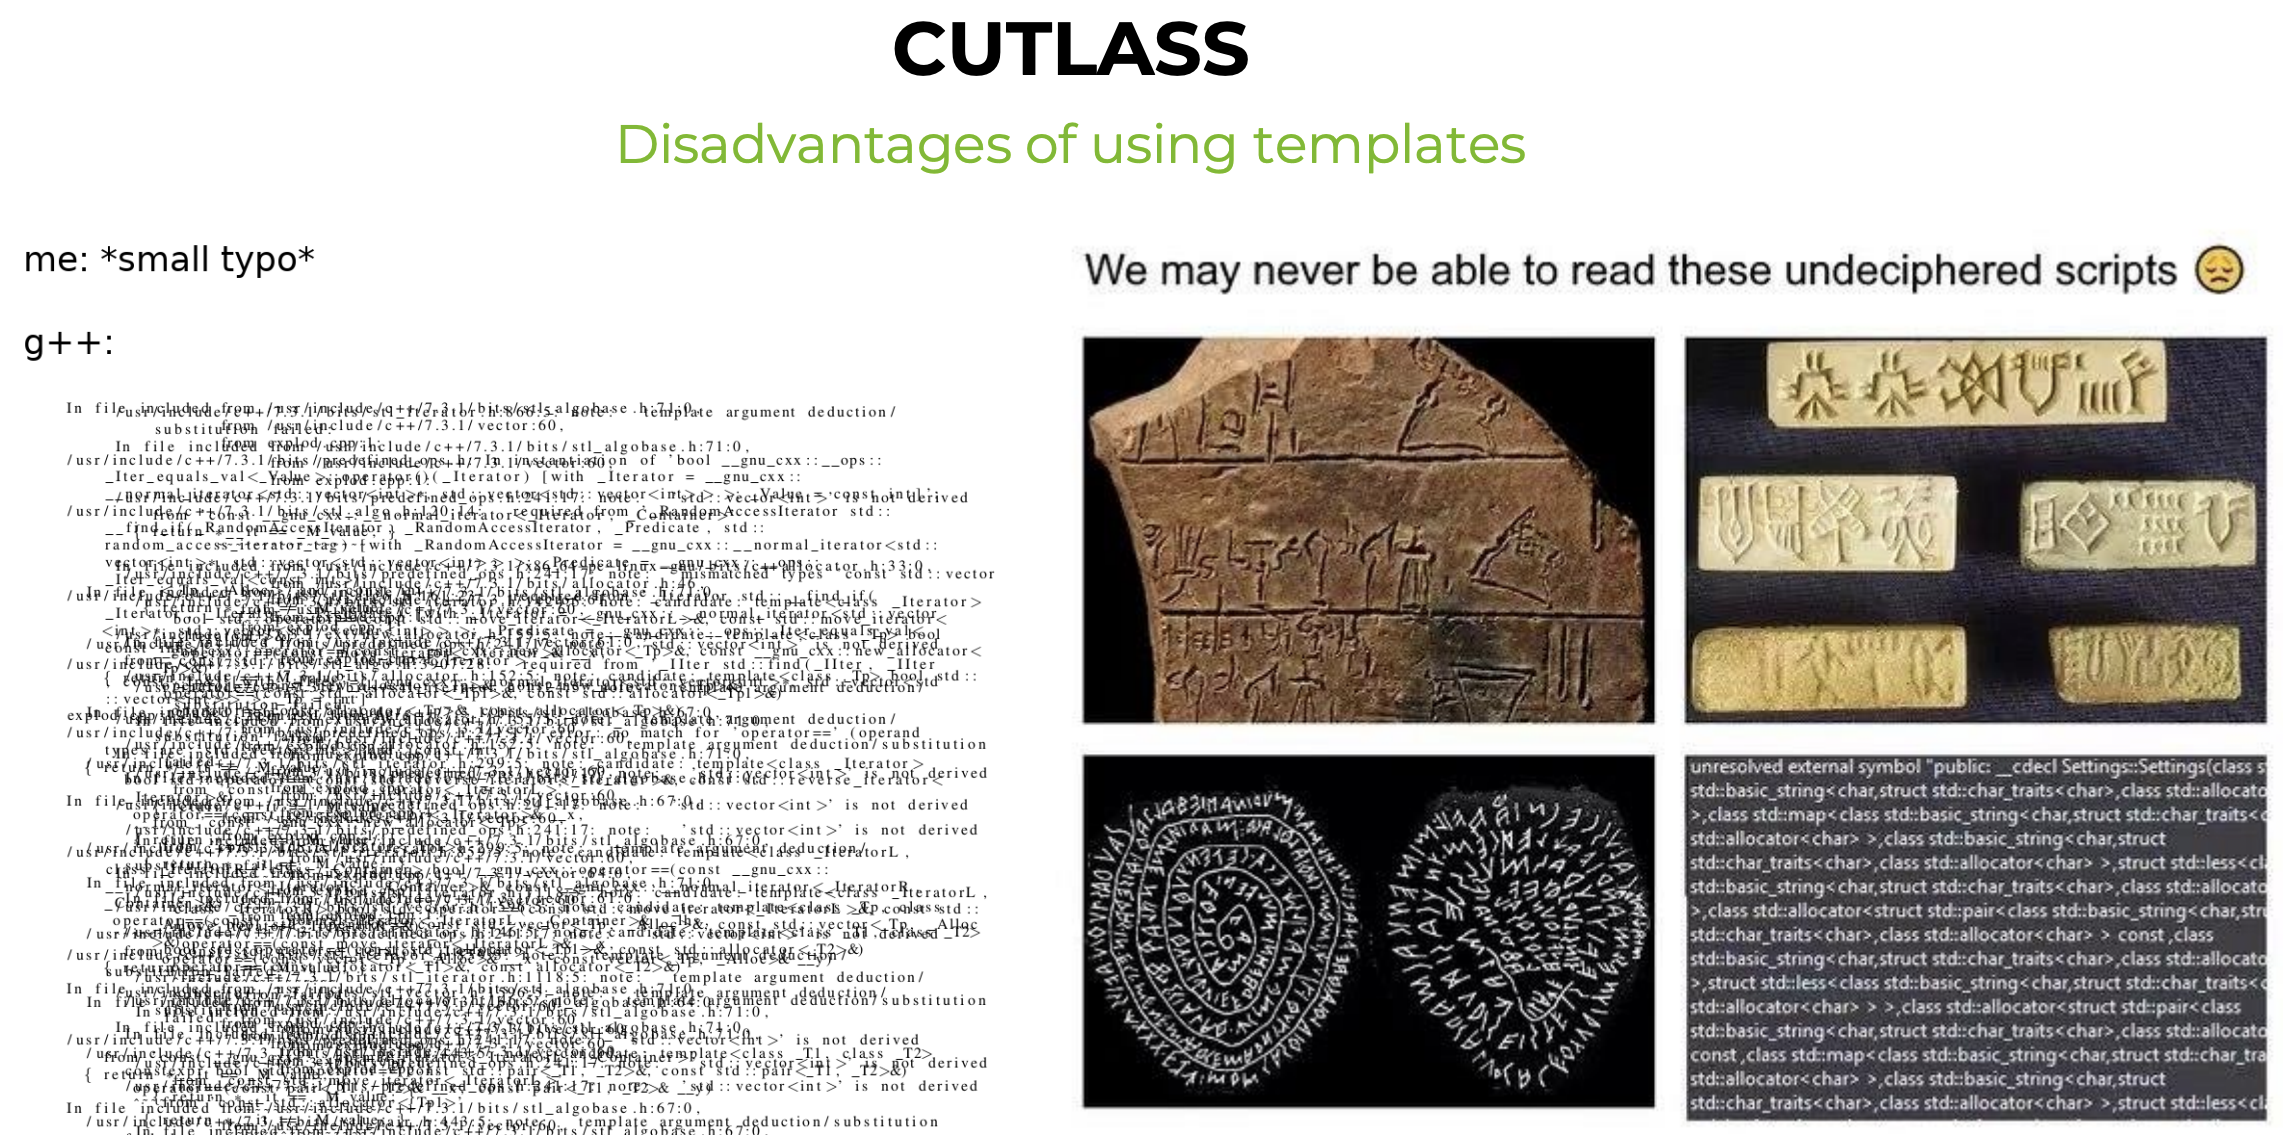
\includegraphics[width=0.8\textwidth]{day8_pm/img/2-templates}
        \caption{Cite: Yoolc's Sharing on CUTLASS}
    \end{figure}
\end{frame}

\subsection{Concurrency Support}
% 按时间引入 C++ 对并行编程的支持
% C++11:Threads, Mutual exclusion, Atomic operations, Condition variables, Futures
% C++20:Cooperative cancellation, Semaphores, Latches and Barriers
\begin{frame}[fragile]{Concurrency support library}
    \begin{itemize}
        \item \textbf{C++11} (We will learn):
              \begin{itemize}
                  \item \texttt{<thread>}: Create and manage threads
                  \item \texttt{<mutex>}: Mutual exclusion for shared data
                  \item \texttt{<atomic>}: Atomic operations for thread safety
                  \item \texttt{<condition\_variable>}: Synchronization between threads
                  \item \texttt{<future>}: Asynchronous results
              \end{itemize}
        \item \textbf{C++20}:
              \begin{itemize}
                  \item \texttt{<stop\_token>}: Cooperative cancellation
                  \item \texttt{<semaphore>}, \texttt{<latch>}, and \texttt{<barrier>}: Advanced synchronization
              \end{itemize}
    \end{itemize}
\end{frame}

%\input{day8_pm/sections/3_parallel_overview}
%\section{Shared Data Synchronization}

\subsection{Race Conditions}
\begin{frame}[fragile]{\emoji{racing-car} Race Condition Demonstration (1/2)}
	\textbf{The Problem}: Multiple threads accessing shared data simultaneously

	\begin{minted}{cpp}
int counter = 0;  // Shared global variable

void increment_unsafe(int iterations) {
    for(int i = 0; i < iterations; i++) {
        counter++;  // NOT thread-safe!
    }
}
	\end{minted}
\end{frame}

\begin{frame}[fragile]{\emoji{racing-car} Race Condition Demonstration (2/2)}
	\textbf{Threading Code}:

	\begin{minted}{cpp}
// Create 4 threads, each incrementing 100000 times
std::vector<std::thread> threads;
for(int i = 0; i < 4; i++) {
    threads.emplace_back(increment_unsafe, 100000);
}

// Wait for completion
for(auto& t : threads) {
    t.join();
}

std::cout << "Expected: 400000" << std::endl;
std::cout << "Actual:   " << counter << std::endl;
	\end{minted}

	\textbf{Expected}: 400000 \quad \textbf{Typical actual}: 387234 (varies!)
\end{frame}

\begin{frame}[fragile]{\emoji{microscope} Why Race Conditions Happen}
	\textbf{Assembly Analysis of} \texttt{counter++}:

	\begin{columns}
		\begin{column}{0.5\textwidth}
			\textbf{C++ Code}
			\begin{minted}{cpp}
counter++;
			\end{minted}

			\vspace{1em}
			\textbf{Assembly (x86-64)}
			\begin{minted}{asm}
mov    eax, DWORD PTR [counter]
add    eax, 1
mov    DWORD PTR [counter], eax
			\end{minted}
		\end{column}
		\begin{column}{0.5\textwidth}
			\textbf{Thread Interleaving}
			\begin{table}[h]
				\tiny
				\begin{tabular}{|l|l|l|}
					\hline
					\textbf{Thread 1}  & \textbf{Thread 2}  & \textbf{counter} \\
					\hline
					mov eax, [counter] &                    & 0                \\
					(eax = 0)          &                    & 0                \\
					                   & mov eax, [counter] & 0                \\
					                   & (eax = 0)          & 0                \\
					add eax, 1         &                    & 0                \\
					(eax = 1)          &                    & 0                \\
					                   & add eax, 1         & 0                \\
					                   & (eax = 1)          & 0                \\
					mov [counter], eax &                    & 1                \\
					                   & mov [counter], eax & 1                \\
					\hline
				\end{tabular}
			\end{table}

			\textbf{Result}: Both threads read 0, both write 1
			\\Expected: 2, Actual: 1
		\end{column}
	\end{columns}

	\vspace{0.5em}
	\textbf{Critical Section}: The portion of code that accesses shared resources
\end{frame}

\subsection{Mutexes and RAII}
\begin{frame}[fragile]{\emoji{lock} From C Mutexes to C++ RAII Locks}
	\begin{columns}
		\begin{column}{0.5\textwidth}
			\textbf{C pthread Mutex}
			\begin{minted}{c}
pthread_mutex_t mutex =
  PTHREAD_MUTEX_INITIALIZER;
void* increment_safe(void* arg) {
    int iterations = *(int*)arg;
    for(int i = 0; i < iterations; i++) {
        pthread_mutex_lock(&mutex);
        counter++;
        pthread_mutex_unlock(&mutex);
    }
    return NULL;
}
// Manual cleanup required
pthread_mutex_destroy(&mutex);
			\end{minted}
		\end{column}
		\begin{column}{0.5\textwidth}
			\textbf{C++ RAII Lock}
			\begin{minted}{cpp}
std::mutex mtx;
void increment_safe(int iterations) {
    for(int i = 0; i < iterations; i++) {
        std::lock_guard<std::mutex>
          lock(mtx);
        counter++;
        // Auto unlock at scope end
    }
}// Automatic cleanup!
			\end{minted}
		\end{column}
	\end{columns}

	\vspace{0.5em}
	\textbf{RAII Benefits}: Exception Safety • No Manual Management • Scope-based
\end{frame}

\begin{frame}[fragile]{\emoji{hammer-and-wrench} Fixed Counter Example (1/2)}
	\begin{minted}{cpp}
std::mutex counter_mutex;
int counter = 0;

void increment_safe(int iterations) {
    for(int i = 0; i < iterations; i++) {
        std::lock_guard<std::mutex> lock(counter_mutex);
        counter++;  // Now thread-safe!
    }
}
	\end{minted}
\end{frame}

\begin{frame}[fragile]{\emoji{hammer-and-wrench} Fixed Counter Example (2/2)}
	\textbf{Usage}:

	\begin{minted}{cpp}
// Same threading code as before
std::vector<std::thread> threads;
for(int i = 0; i < 4; i++) {
    threads.emplace_back(increment_safe, 100000);
}

for(auto& t : threads) {
    t.join();
}

std::cout << "Expected: 400000" << std::endl;
std::cout << "Actual:   " << counter << std::endl;
// Result: Success: Y (always!)
	\end{minted}
\end{frame}

\subsection{Deadlock Prevention}
\begin{frame}[fragile]{\emoji{skull} Deadlock: The Four Horsemen}
	\textbf{Deadlock Conditions} (All must be present):
	\begin{enumerate}
		\item \textbf{Mutual Exclusion}: Resources cannot be shared
		\item \textbf{Hold and Wait}: Process holds resource while waiting for another
		\item \textbf{No Preemption}: Resources cannot be forcibly taken
		\item \textbf{Circular Wait}: Circular chain of waiting processes
	\end{enumerate}

	\vspace{1em}
	\textbf{Classic Deadlock Example}:
	\begin{minted}{cpp}
std::mutex mutex1, mutex2;
void thread1() {
    std::lock_guard<std::mutex> lock1(mutex1);
    std::this_thread::sleep_for(std::chrono::milliseconds(10));
    std::lock_guard<std::mutex> lock2(mutex2);  // Waits forever
    // Do work...
}
void thread2() {
    std::lock_guard<std::mutex> lock2(mutex2);
    std::this_thread::sleep_for(std::chrono::milliseconds(10));
    std::lock_guard<std::mutex> lock1(mutex1);  // Waits forever
    // Do work...
}
	\end{minted}

	\emoji{warning} \textbf{Result}: Both threads wait forever!
\end{frame}

\begin{frame}[fragile]{\emoji{shield} Deadlock Prevention: Strategy 1}
	\textbf{Ordered Locking}

	\begin{minted}{cpp}
std::mutex mutex1, mutex2;

void thread1() {
    std::lock_guard<std::mutex> lock1(mutex1);  // Same order
    std::lock_guard<std::mutex> lock2(mutex2);
    // Do work...
}

void thread2() {
    std::lock_guard<std::mutex> lock1(mutex1);  // Same order
    std::lock_guard<std::mutex> lock2(mutex2);
    // Do work...
}
	\end{minted}
\end{frame}

\begin{frame}[fragile]{\emoji{shield} Deadlock Prevention: Strategy 2}
	\textbf{Atomic Multi-lock}

	\begin{minted}{cpp}
void thread1() {
    std::unique_lock<std::mutex> lock1(mutex1, std::defer_lock);
    std::unique_lock<std::mutex> lock2(mutex2, std::defer_lock);

    std::lock(lock1, lock2);  // Atomic acquisition
    // Do work...
}  // Automatic release

void thread2() {
    // ... same pattern ...
    std::lock(lock1, lock2);  // Same atomic acquisition
}
	\end{minted}
\end{frame}

\begin{frame}[fragile]{\emoji{bank} Bank Transfer: Class Definition}
	\begin{minted}{cpp}
class BankAccount {
private:
    double balance;
    mutable std::mutex mtx;

public:
    BankAccount(double initial) : balance(initial) {}

    double get_balance() const {
        std::lock_guard<std::mutex> lock(mtx);
        return balance;
    }

    // Safe transfer using ordered locking
    static void transfer(BankAccount& from, BankAccount& to,
                        double amount);
};
	\end{minted}
\end{frame}

\begin{frame}[fragile]{\emoji{bank} Bank Transfer: Implementation}
	\begin{minted}{cpp}
void BankAccount::transfer(BankAccount& from, BankAccount& to,
                          double amount) {
    // Prevent deadlock with consistent lock ordering
    if (&from < &to) {
        std::lock_guard<std::mutex> lock1(from.mtx);
        std::lock_guard<std::mutex> lock2(to.mtx);
        from.balance -= amount;
        to.balance += amount;
    } else {
        std::lock_guard<std::mutex> lock1(to.mtx);
        std::lock_guard<std::mutex> lock2(from.mtx);
        from.balance -= amount;
        to.balance += amount;
    }
}

// Usage: BankAccount::transfer(alice, bob, 100);
	\end{minted}
\end{frame}

%\section{Producer-Consumer Model}

\subsection{The Need for Condition Variables}
\begin{frame}[fragile]{\emoji{sleeping} Why Not Just Use Busy-Waiting?}
	\textbf{Naive Approach: Polling}
	\begin{minted}{cpp}
std::queue<int> buffer;
std::mutex buffer_mutex;
bool done = false;

void consumer_busy_wait() {
    while (!done) {
        std::lock_guard<std::mutex> lock(buffer_mutex);
        if (!buffer.empty()) {
            int item = buffer.front();
            buffer.pop();
            std::cout << "Consumed: " << item << std::endl;
        }
        // Busy waiting - wastes CPU cycles!
    }
}
	\end{minted}

	\textbf{Problems}: CPU Waste • Power Drain • Lock Contention • Poor Scalability

	\emoji{bulb} \textbf{Solution}: Condition Variables - Sleep until notified!
\end{frame}

\subsection{Condition Variables}
\begin{frame}[fragile]{\emoji{bell} Condition Variables: Efficient Waiting}
	\textbf{Core Operations}:
	\begin{itemize}
		\item \texttt{wait(lock, predicate)}: Sleep until condition is true
		\item \texttt{notify\_one()}: Wake up one waiting thread
		\item \texttt{notify\_all()}: Wake up all waiting threads
	\end{itemize}

	\vspace{0.5em}
	\textbf{Basic Pattern}:
	\begin{minted}{cpp}
std::mutex mtx;
std::condition_variable cv;
bool ready = false;

void waiter() {
    std::unique_lock<std::mutex> lock(mtx);
    cv.wait(lock, []{ return ready; });  // Sleep until ready
    std::cout << "Condition met!" << std::endl;
}

void notifier() {
    {
        std::lock_guard<std::mutex> lock(mtx);
        ready = true;  // Set condition
    }
    cv.notify_one();  // Wake up waiter
}
	\end{minted}

	\textbf{Key Points}: Use \texttt{unique\_lock} • Always use predicate • Modify before notify
\end{frame}

\begin{frame}[fragile]{\emoji{gear} How Condition Variables Work}
	\textbf{Internal Mechanism}:

	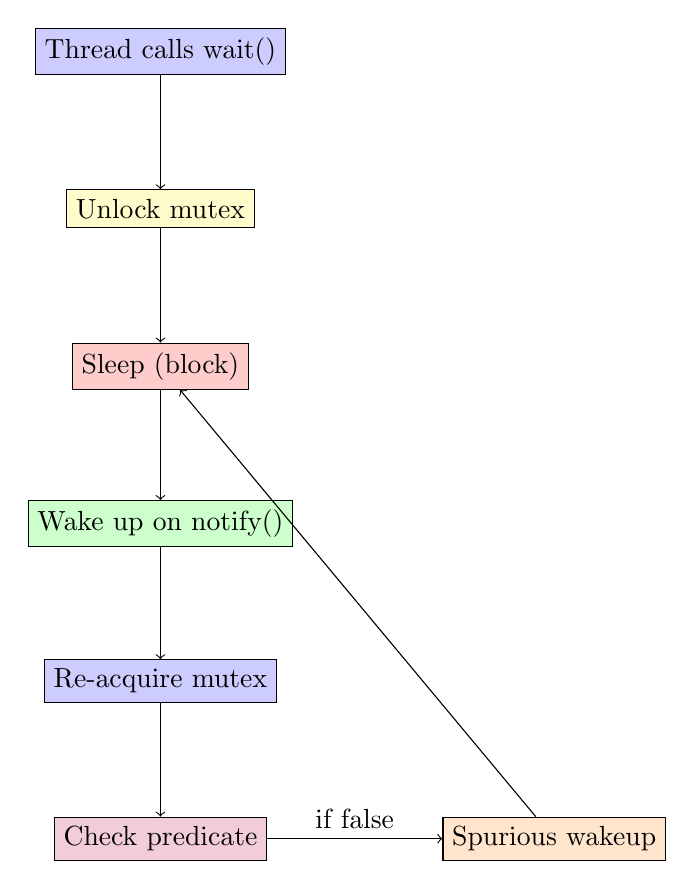
\begin{tikzpicture}[node distance=2cm]
		% Nodes
		\node[draw, rectangle, fill=blue!20] (thread) {Thread calls wait()};
		\node[draw, rectangle, fill=yellow!20, below of=thread] (unlock) {Unlock mutex};
		\node[draw, rectangle, fill=red!20, below of=unlock] (sleep) {Sleep (block)};
		\node[draw, rectangle, fill=green!20, below of=sleep] (wakeup) {Wake up on notify()};
		\node[draw, rectangle, fill=blue!20, below of=wakeup] (relock) {Re-acquire mutex};
		\node[draw, rectangle, fill=purple!20, below of=relock] (check) {Check predicate};
		\node[draw, rectangle, fill=orange!20, right of=check, xshift=3cm] (spurious) {Spurious wakeup};

		% Arrows
		\draw[->] (thread) -- (unlock);
		\draw[->] (unlock) -- (sleep);
		\draw[->] (sleep) -- (wakeup);
		\draw[->] (wakeup) -- (relock);
		\draw[->] (relock) -- (check);
		\draw[->] (check) -- node[above] {if false} (spurious);
		\draw[->] (spurious) -- (sleep);
	\end{tikzpicture}

	\vspace{0.5em}
	\textbf{Why Use Predicates?}
	\begin{minted}{cpp}
// Vulnerable to spurious wakeups
cv.wait(lock);
if (condition) { /* work */ }

// Robust against spurious wakeups
cv.wait(lock, []{ return condition; });
// Equivalent to:
while (!condition) {
    cv.wait(lock);
}
	\end{minted}
\end{frame}

\subsection{Thread-Safe Queue Implementation}
\begin{frame}[fragile]{\emoji{package} Thread-Safe Queue: Structure}
	\textbf{Class Definition}:

	\begin{minted}{cpp}
template<typename T>
class ThreadSafeQueue {
private:
    std::queue<T> queue_;
    mutable std::mutex mutex_;
    std::condition_variable condition_;

public:
    void push(const T& item);
    T pop();  // Blocks until item available
    bool empty() const;
    size_t size() const;
};
	\end{minted}
\end{frame}

\begin{frame}[fragile]{\emoji{package} Thread-Safe Queue: Implementation}
	\textbf{Core Methods}:

	\begin{minted}{cpp}
void push(const T& item) {
    {
        std::lock_guard<std::mutex> lock(mutex_);
        queue_.push(item);
    }
    condition_.notify_one();  // Wake up waiting consumers
}

T pop() {
    std::unique_lock<std::mutex> lock(mutex_);
    condition_.wait(lock, [this] { return !queue_.empty(); });

    T item = queue_.front();
    queue_.pop();
    return item;
}
	\end{minted}
\end{frame}

\subsection{Producer-Consumer Implementation}
\begin{frame}[fragile]{\emoji{factory} Producer-Consumer: Simplified Example}
	\begin{minted}{cpp}
ThreadSafeQueue<int> shared_queue;
bool done = false;

void producer(int id, int num_items) {
    for (int i = 0; i < num_items; ++i) {
        int item = rand() % 100;
        shared_queue.push(item);
        std::cout << "Producer " << id << " produced: " << item << std::endl;

        std::this_thread::sleep_for(std::chrono::milliseconds(100));
    }
}

void consumer(int id) {
    while (!done) {
        int item = shared_queue.pop();  // Blocks until available
        std::cout << "Consumer " << id << " consumed: " << item << std::endl;

        std::this_thread::sleep_for(std::chrono::milliseconds(150));
    }
}
	\end{minted}
\end{frame}

\begin{frame}[fragile]{\emoji{rocket} Running the System}
	\begin{minted}{cpp}
int main() {
    std::vector<std::thread> threads;

    // Start 3 consumers
    for (int i = 0; i < 3; ++i) {
        threads.emplace_back(consumer, i);
    }

    // Start 2 producers
    for (int i = 0; i < 2; ++i) {
        threads.emplace_back(producer, i, 5);  // 5 items each
    }

    // Wait for producers to finish (simplified)
    std::this_thread::sleep_for(std::chrono::seconds(3));
    done = true;  // Signal consumers to stop

    // Wait for all threads
    for (auto& t : threads) {
        t.join();
    }

    return 0;
}
	\end{minted}

	\textbf{Benefits}: Efficient waiting • No busy loops • Thread-safe communication
\end{frame}

\begin{frame}[fragile]{\emoji{chart-increasing} Performance Comparison}
	\textbf{Busy-Waiting vs Condition Variables}

	\begin{table}[h]
		\centering
		\begin{tabular}{|l|c|c|}
			\hline
			\textbf{Metric}   & \textbf{Busy-Waiting} & \textbf{Condition Variables} \\
			\hline
			CPU Usage         & 95-100\%              & 5-15\%                       \\
			Response Time     & Low                   & Low                          \\
			Throughput        & Medium                & High                         \\
			Power Consumption & High                  & Low                          \\
			Scalability       & Poor                  & Good                         \\
			\hline
		\end{tabular}
	\end{table}

	\vspace{1em}
	\textbf{Real-world Applications}:
	\begin{itemize}
		\item \textbf{Web Servers}: Request queue processing
		\item \textbf{Database Systems}: Transaction queue management
		\item \textbf{Game Engines}: Event processing pipelines
		\item \textbf{Media Players}: Audio/video buffer management
	\end{itemize}
\end{frame}

%\section{Summary and Framework Selection}

\subsection{Core Concepts Review}
\begin{frame}[fragile]{\emoji{brain} C++ Concurrency Core Concepts}
	\textbf{The Three Pillars}:

	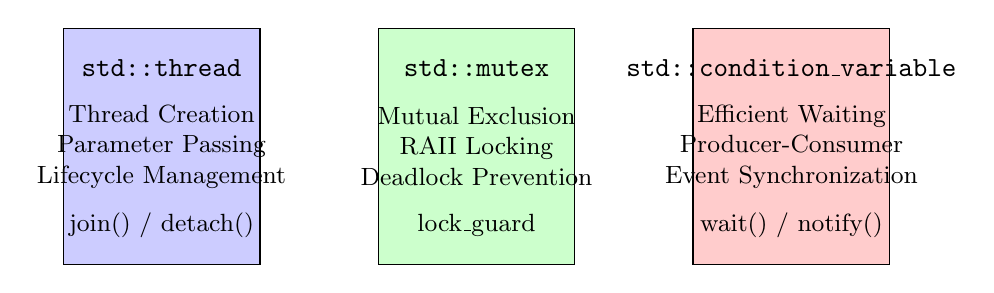
\begin{tikzpicture}
		% Pillar 1: Thread
		\node[draw, rectangle, fill=blue!20, minimum height=3cm, minimum width=2.5cm] (thread) at (0,0) {};
		\node[font=\bfseries] at (0,1) {\texttt{std::thread}};
		\node[font=\small, align=center] at (0,0) {Thread Creation\\Parameter Passing\\Lifecycle Management};
		\node[font=\small] at (0,-1) {join() / detach()};

		% Pillar 2: Mutex
		\node[draw, rectangle, fill=green!20, minimum height=3cm, minimum width=2.5cm] (mutex) at (4,0) {};
		\node[font=\bfseries] at (4,1) {\texttt{std::mutex}};
		\node[font=\small, align=center] at (4,0) {Mutual Exclusion\\RAII Locking\\Deadlock Prevention};
		\node[font=\small] at (4,-1) {lock\_guard};

		% Pillar 3: Condition Variable
		\node[draw, rectangle, fill=red!20, minimum height=3cm, minimum width=2.5cm] (cv) at (8,0) {};
		\node[font=\bfseries] at (8,1) {\texttt{std::condition\_variable}};
		\node[font=\small, align=center] at (8,0) {Efficient Waiting\\Producer-Consumer\\Event Synchronization};
		\node[font=\small] at (8,-1) {wait() / notify()};
	\end{tikzpicture}

	\vspace{2em}
	\textbf{Best Practices Checklist}:
	\begin{itemize}
		\item \emoji{check-mark} Always join() or detach() threads
		\item \emoji{check-mark} Use RAII locks (\texttt{lock\_guard}, \texttt{unique\_lock})
		\item \emoji{check-mark} Avoid deadlocks with ordered locking
		\item \emoji{check-mark} Use condition variables instead of busy-waiting
		\item \emoji{check-mark} Pass by value or \texttt{std::ref} explicitly
	\end{itemize}
\end{frame}

\subsection{Framework Selection Guide}
\begin{frame}[fragile]{\emoji{compass} When to Choose Which Framework}
	\begin{tikzpicture}[node distance=1.5cm]
		% Decision tree
		\node[draw, diamond, fill=yellow!20] (start) {Parallel Task};

		\node[draw, diamond, below left of=start, fill=blue!10] (pattern) {Regular Pattern?};
		\node[draw, diamond, below right of=start, fill=blue!10] (scale) {Scale Requirement?};

		\node[draw, rectangle, below of=pattern, fill=green!20] (openmp) {OpenMP};
		\node[draw, rectangle, below left of=scale, fill=red!20] (cpp) {C++ Thread};
		\node[draw, rectangle, below right of=scale, fill=purple!20] (mpi) {MPI};

		% Arrows with labels
		\draw[->] (start) -- node[above left] {Data Parallel} (pattern);
		\draw[->] (start) -- node[above right] {Task Parallel} (scale);
		\draw[->] (pattern) -- node[left] {Yes} (openmp);
		\draw[->] (scale) -- node[above left] {Single Node} (cpp);
		\draw[->] (scale) -- node[above right] {Multi-node} (mpi);
	\end{tikzpicture}

	\vspace{1em}
	\textbf{Detailed Comparison}:
	\begin{table}[h]
		\centering
		\tiny
		\begin{tabular}{|l|c|c|c|}
			\hline
			\textbf{Criteria}    & \textbf{OpenMP} & \textbf{C++ Thread} & \textbf{MPI} \\
			\hline
			Learning Curve       & Easy            & Moderate            & Hard         \\
			Development Time     & Fast            & Medium              & Slow         \\
			Performance Control  & Low             & High                & High         \\
			Debugging Complexity & Low             & Medium              & High         \\
			Memory Model         & Shared          & Shared              & Distributed  \\
			Scalability          & 1-64 cores      & 1-32 cores          & 1000s cores  \\
			\hline
			\textbf{Best For}    & Loops           & Complex Logic       & HPC Clusters \\
			\hline
		\end{tabular}
	\end{table}
\end{frame}

\subsection{Comprehensive Example}
\begin{frame}[fragile]{\emoji{dart} Monte Carlo π Calculation: All Frameworks}
	\textbf{Problem}: Estimate π using random point sampling

	\begin{columns}
		\begin{column}{0.3\textwidth}
			\textbf{OpenMP Version}
			\begin{minted}{cpp}
#include <omp.h>
#include <random>

double monte_carlo_openmp(long samples) {
    long count = 0;

    #pragma omp parallel reduction(+:count)
    {
        std::random_device rd;
        std::mt19937 gen(rd());
        std::uniform_real_distribution<> dis(0.0, 1.0);

        #pragma omp for
        for(long i = 0; i < samples; i++) {
            double x = dis(gen);
            double y = dis(gen);
            if(x*x + y*y <= 1.0) {
                count++;
            }
        }
    }

    return 4.0 * count / samples;
}
			\end{minted}
		\end{column}
		\begin{column}{0.35\textwidth}
			\textbf{C++ Thread Version}
			\begin{minted}{cpp}
#include <thread>
#include <vector>
#include <atomic>

std::atomic<long> global_count(0);

void worker(long samples) {
    std::random_device rd;
    std::mt19937 gen(rd());
    std::uniform_real_distribution<> dis(0.0, 1.0);

    long local_count = 0;
    for(long i = 0; i < samples; i++) {
        double x = dis(gen);
        double y = dis(gen);
        if(x*x + y*y <= 1.0) {
            local_count++;
        }
    }

    global_count += local_count;
}

double monte_carlo_cpp(long samples) {
    const int num_threads = std::thread::hardware_concurrency();
    std::vector<std::thread> threads;

    long samples_per_thread = samples / num_threads;

    for(int i = 0; i < num_threads; i++) {
        threads.emplace_back(worker, samples_per_thread);
    }

    for(auto& t : threads) {
        t.join();
    }

    return 4.0 * global_count / samples;
}
			\end{minted}
		\end{column}
		\begin{column}{0.35\textwidth}
			\textbf{MPI Version}
			\begin{minted}{cpp}
#include <mpi.h>

double monte_carlo_mpi(long samples) {
    int rank, size;
    MPI_Comm_rank(MPI_COMM_WORLD, &rank);
    MPI_Comm_size(MPI_COMM_WORLD, &size);

    long local_samples = samples / size;
    long local_count = 0;

    std::random_device rd;
    std::mt19937 gen(rd() + rank);
    std::uniform_real_distribution<> dis(0.0, 1.0);

    for(long i = 0; i < local_samples; i++) {
        double x = dis(gen);
        double y = dis(gen);
        if(x*x + y*y <= 1.0) {
            local_count++;
        }
    }

    long global_count;
    MPI_Reduce(&local_count, &global_count, 1,
               MPI_LONG, MPI_SUM, 0, MPI_COMM_WORLD);

    if(rank == 0) {
        return 4.0 * global_count / samples;
    }
    return 0.0;
}
			\end{minted}
		\end{column}
	\end{columns}
\end{frame}

\begin{frame}[fragile]{\emoji{bar-chart} Performance Analysis}
	\textbf{Benchmark Results} (1 billion samples):

	\begin{table}[h]
		\centering
		\begin{tabular}{|l|c|c|c|c|}
			\hline
			\textbf{Framework} & \textbf{Time (s)} & \textbf{Speedup} & \textbf{Accuracy} & \textbf{LOC} \\
			\hline
			Sequential         & 12.5              & 1.0×             & π ≈ 3.141592      & 15           \\
			OpenMP             & 1.8               & 6.9×             & π ≈ 3.141591      & 20           \\
			C++ Thread         & 1.9               & 6.6×             & π ≈ 3.141593      & 35           \\
			MPI (8 nodes)      & 0.3               & 41.7×            & π ≈ 3.141590      & 40           \\
			\hline
		\end{tabular}
	\end{table}

	\vspace{1em}
	\textbf{Trade-offs Analysis}:
	\begin{itemize}
		\item \textbf{OpenMP}: Best effort/performance ratio for shared memory
		\item \textbf{C++ Thread}: Maximum control, good for complex algorithms
		\item \textbf{MPI}: Unmatched scalability for distributed computing
	\end{itemize}

	\vspace{0.5em}
	\textbf{Development Productivity}:
	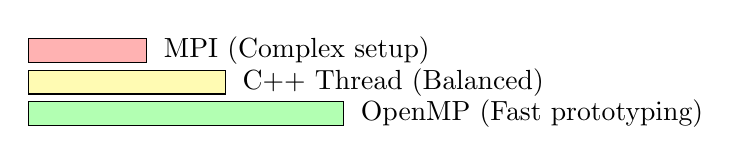
\begin{tikzpicture}
		\draw[fill=green!30] (0,0) rectangle (4,0.3);
		\draw[fill=yellow!30] (0,0.4) rectangle (2.5,0.7);
		\draw[fill=red!30] (0,0.8) rectangle (1.5,1.1);

		\node[right] at (4.1,0.15) {OpenMP (Fast prototyping)};
		\node[right] at (2.6,0.55) {C++ Thread (Balanced)};
		\node[right] at (1.6,0.95) {MPI (Complex setup)};
	\end{tikzpicture}
\end{frame}

\subsection{Advanced Topics Preview}
\begin{frame}[fragile]{\emoji{telescope} Beyond the Basics: Advanced Concurrency}
	\textbf{Topics for Further Exploration}:

	\begin{columns}
		\begin{column}{0.5\textwidth}
			\textbf{Asynchronous Programming}
			\begin{minted}{cpp}
#include <future>

auto future = std::async(std::launch::async,
    []() {
        return expensive_computation();
    });

// Do other work...
auto result = future.get();  // Wait for result
			\end{minted}

			\textbf{Atomic Operations}
			\begin{minted}{cpp}
#include <atomic>

std::atomic<int> counter{0};

void increment() {
    counter.fetch_add(1, std::memory_order_relaxed);
}
			\end{minted}
		\end{column}
		\begin{column}{0.5\textwidth}
			\textbf{Thread Pools}
			\begin{minted}{cpp}
class ThreadPool {
    std::vector<std::thread> workers;
    std::queue<std::function<void()>> tasks;
    std::mutex queue_mutex;
    std::condition_variable condition;

public:
    template<class F>
    void enqueue(F&& f) {
        {
            std::lock_guard<std::mutex> lock(queue_mutex);
            tasks.emplace(std::forward<F>(f));
        }
        condition.notify_one();
    }
};
			\end{minted}
		\end{column}
	\end{columns}

	\vspace{1em}
	\textbf{Learning Path}:
	\begin{enumerate}
		\item Master the basics: \texttt{thread}, \texttt{mutex}, \texttt{condition\_variable}
		\item Explore \texttt{std::async} and \texttt{std::future}
		\item Study atomic operations and memory models
		\item Implement lock-free data structures
		\item Build thread pools and work-stealing algorithms
	\end{enumerate}
\end{frame}

%
%\begin{frame}[fragile]{Takeaways}
%	\emoji{star} Important concepts that you should remember today:
%	\begin{itemize}
%		\item \textbf{C++ Concurrency Trinity}: \texttt{std::thread}, \texttt{std::mutex}, \texttt{std::condition\_variable}
%		\item \textbf{RAII Principle}: Automatic resource management with lock guards
%		\item \textbf{Producer-Consumer Pattern}: Efficient thread communication
%		\item \textbf{Framework Selection}: Choose the right tool for the right job
%	\end{itemize}
%\end{frame}
%
%% Q&A
%\begin{frame}[standout]
%	\Huge\textsc{Thank You}
%
%	\vfill
%
%	\LARGE\textsc{Any Questions?}
%\end{frame}

\end{document}
